\documentclass{beamer}
\usetheme{Madrid}
\usepackage[T1]{fontenc}
\usepackage{mathpazo}
\usepackage{graphicx}
\usepackage{booktabs}
\usepackage{tikz}
\usetikzlibrary{positioning,arrows.meta,shapes.geometric,fit,backgrounds,calc}
\definecolor{cetnavy}{RGB}{10,26,63}
\definecolor{cetlight}{RGB}{225,231,242}
\setbeamercolor{structure}{fg=cetnavy}
\setbeamercolor{frametitle}{bg=cetnavy,fg=white}
\setbeamercolor{title}{bg=cetnavy,fg=white}
\setbeamertemplate{navigation symbols}{}
% =====================================================================
%  EDIT YOUR DETAILS HERE — this ONE file feeds every abstract & deck.
%  (Change a value, recompile; all 36 documents update.)
% =====================================================================
\newcommand{\seminarName}{Aflah Muhammed P}      % <-- your full name (guessed from your email; please verify)
\newcommand{\seminarRoll}{TVE00CS000}            % <-- your university register/roll number
\newcommand{\seminarClassRoll}{00}               % <-- your class roll no (the short one)
\newcommand{\seminarGuide}{Prof.\ <Guide Name>}  % <-- your guide
\newcommand{\seminarDept}{Department of Computer Science and Engineering}
\newcommand{\seminarCollege}{College of Engineering Trivandrum}
\newcommand{\seminarShortCollege}{CET}           % shown in the slide footer, e.g. "Aflah Muhammed P (CET)"
\newcommand{\seminarShortTitle}{B.Tech Seminar}  % middle of the slide footer
\newcommand{\seminarDate}{July 31, 2026}
% ---------------------------------------------------------------------
% Optional: put a logo image named  cet_logo.png  in this folder and it
% will appear on every title slide automatically. If absent, it is skipped.
% =====================================================================

\title[\seminarShortTitle]{APIGen-MT: Generating Multi-Turn Tool-Use Data via Agent-Human Simulation}
\author[\seminarName\ (\seminarShortCollege)]{\seminarName \\ \seminarRoll \\ Roll No: \seminarClassRoll \\ Guide: \seminarGuide}
\institute[\seminarShortCollege]{\seminarDept \\ \seminarCollege}
\date{\seminarDate}
\titlegraphic{\IfFileExists{cet_logo.png}{\includegraphics[height=1.1cm]{cet_logo.png}}{}}
\begin{document}
\begin{frame}\titlepage\end{frame}
\begin{frame}{Table of Contents}\tableofcontents\end{frame}
\section{Introduction}
\begin{frame}{Introduction}
\textbf{\textit{Agents that use tools need multi-turn data}}
\begin{itemize}
\item LLM agents call external APIs to solve real tasks.
\item Real tasks are interactive, stateful, multi-turn.
\item Users reveal intent gradually across the dialogue.
\item Training needs verified multi-turn tool-use trajectories.
\item Such data is scarce, costly, and hard to check.
\item APIGen-MT synthesizes it via an agentic pipeline.
\end{itemize}
\end{frame}

\section{Literature Survey}
\begin{frame}{Literature Survey}
\textbf{\textit{Prior work on tool-use data and benchmarks}}
\begin{itemize}
\item APIGen: single-turn verifiable function-calling data.
\item ToolLLM, ToolACE: large tool-use instruction sets.
\item $\tau$-bench: tool-agent-user interaction benchmark.
\item BFCL: Berkeley Function-Calling Leaderboard.
\item xLAM: prior Large Action Model family.
\item Human annotation: expensive and inconsistent.
\end{itemize}
\end{frame}

\section{Motivation}
\begin{frame}{Motivation}
\textbf{\textit{Why existing data pipelines fall short}}
\begin{itemize}
\item Single-turn data ignores dialogue dynamics.
\item Human collection is slow, noisy, unscalable.
\item Long-horizon tasks need verified ground truth.
\item Naive simulation drifts without correctness checks.
\item Goal: scalable data that is provably correct.
\end{itemize}
\end{frame}

\section{Problem Statement}
\begin{frame}{Problem Statement}
\textbf{\textit{The precise problem addressed}}
\begin{itemize}
\item Generate multi-turn tool-use trajectories at scale.
\item Guarantee correctness against ground-truth actions.
\item Capture realistic, incremental human-agent dialogue.
\item Avoid costly, inconsistent human annotation.
\end{itemize}
\end{frame}

\section{Objectives}
\begin{frame}{Objectives / Contributions}
\textbf{\textit{What the paper delivers}}
\begin{itemize}
\item A two-phase agentic data-generation pipeline.
\item Verified task blueprints via a reviewer committee.
\item Faithful agent-human trajectory simulation.
\item Open xLAM-2 models and APIGen-MT-5k data.
\item State-of-the-art multi-turn tool-use performance.
\end{itemize}
\end{frame}

\section{Methodology Overview}
\begin{frame}{Methodology Overview}
\begin{center}
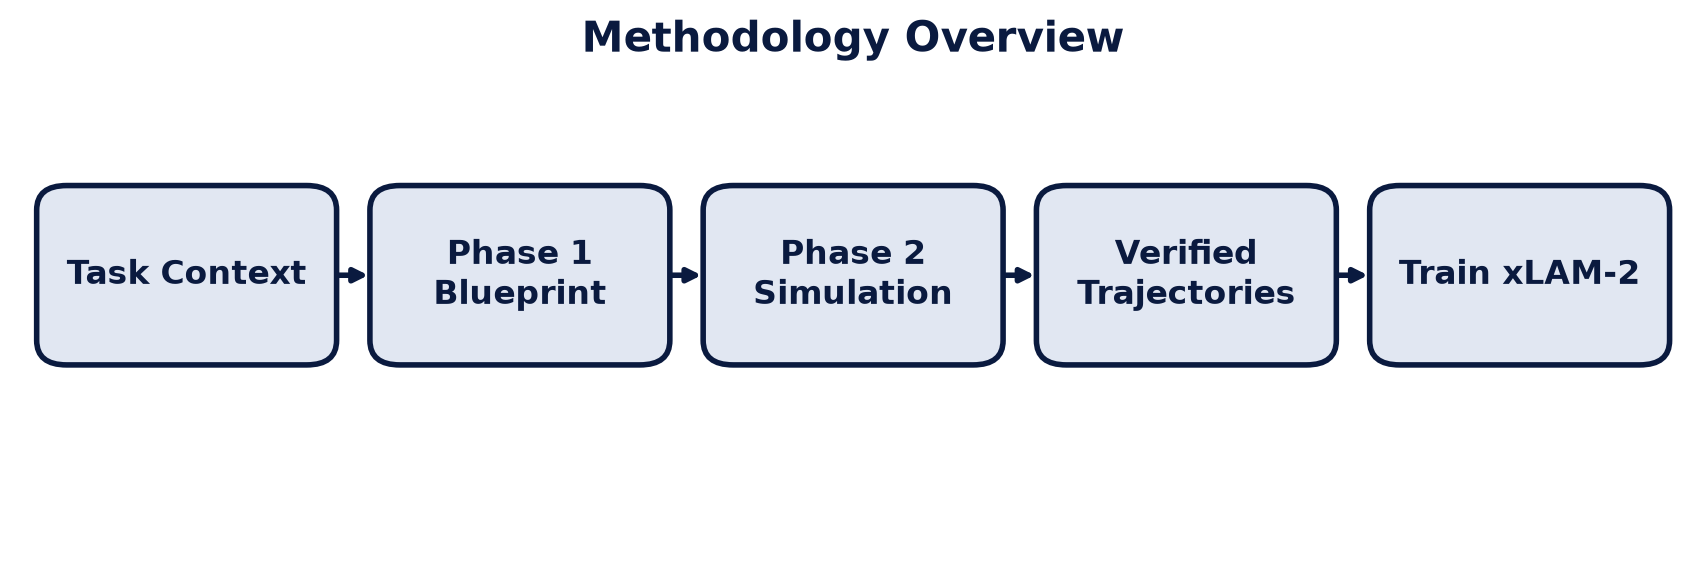
\includegraphics[width=0.9\textwidth,height=0.62\textheight,keepaspectratio]{images/apigenmt_1.png}
\end{center}
\vspace{2mm}
\footnotesize Two phases: verify blueprints first, then realise conversations.
\end{frame}

\begin{frame}{Methodology Overview: Two Phases}
\textbf{\textit{Verification-first design}}
\begin{itemize}
\item Phase 1 fixes ground truth before any dialogue.
\item Reviewer committee rejects low-quality blueprints.
\item Phase 2 turns blueprints into conversations.
\item Only trajectories matching ground truth are kept.
\end{itemize}
\end{frame}

\section{System Architecture}
\begin{frame}{System Architecture: Phase 1 Blueprint Engine}
\begin{center}
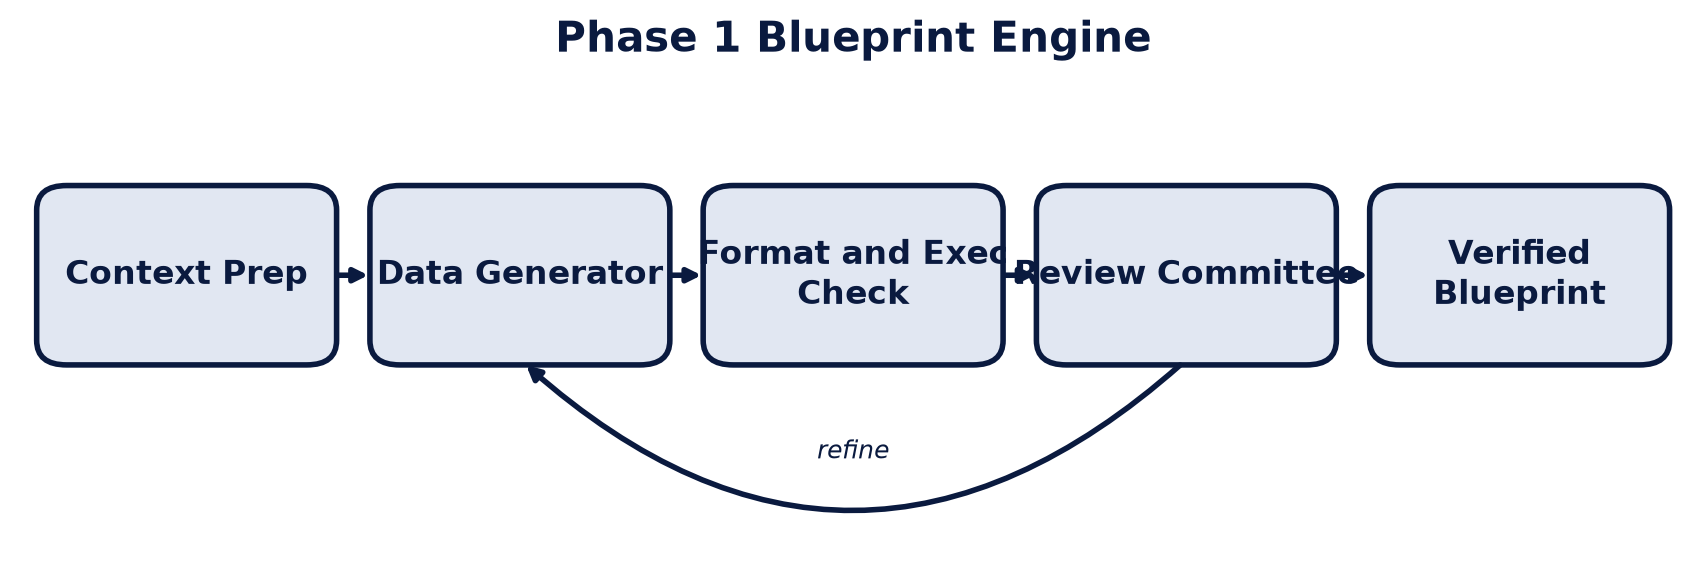
\includegraphics[width=0.9\textwidth,height=0.62\textheight,keepaspectratio]{images/apigenmt_2.png}
\end{center}
\vspace{1mm}
\footnotesize Iterative feedback loop refines rejected candidates until validated.
\end{frame}

\section{Data Collection}
\begin{frame}{Data Collection}
\textbf{\textit{Environments and released data}}
\begin{itemize}
\item Executable domains: retail and airline APIs.
\item Sandbox environments enforce action correctness.
\item Simulated user reveals task details incrementally.
\item 5,000 verified trajectories collected end-to-end.
\item Released publicly as APIGen-MT-5k on Hugging Face.
\end{itemize}
\end{frame}

\section{Model Development}
\begin{frame}{Model Development}
\textbf{\textit{The xLAM-2-fc-r family}}
\begin{itemize}
\item Base: Llama 3.1/3.2 and Qwen 2.5 Instruct.
\item Sizes: 1B, 3B, 8B, 32B, 70B parameters.
\item Fine-tuned on APIGen-MT trajectories.
\item Function-calling and multi-turn agent behaviour.
\item Smaller models often beat larger baselines.
\end{itemize}
\end{frame}

\section{Results}
\begin{frame}{Results: Beating Frontier Models}
\begin{center}
\begin{tabular}{lcc}
\toprule
Model & $\tau$-bench & BFCL v3 \\
\midrule
GPT-4o & 52.9 & 72.08 \\
Claude 3.5 Sonnet & 60.1 & -- \\
xLAM-2-8b-fc-r & -- & 72.83 \\
xLAM-2-70b-fc-r & 56.2 & 78.19 \\
\bottomrule
\end{tabular}
\end{center}
\vspace{2mm}
\footnotesize All values in \%. xLAM-2-70b ranks \#1 on BFCL v3; 8B model already exceeds GPT-4o.
\end{frame}

\begin{frame}{Results: $\tau$-bench Overall Success}
\begin{center}
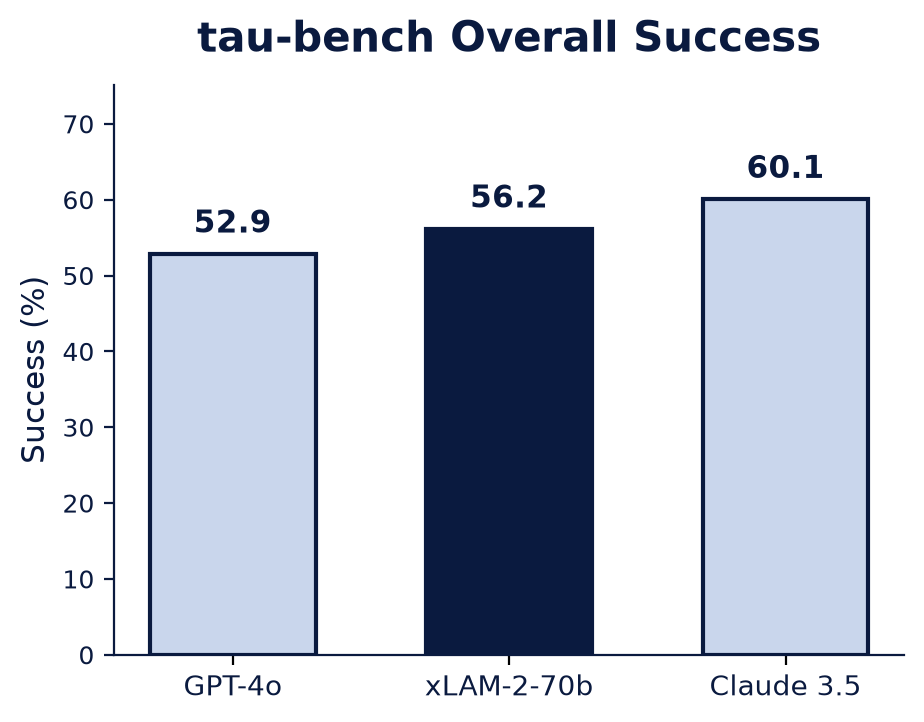
\includegraphics[width=0.9\textwidth,height=0.62\textheight,keepaspectratio]{images/apigenmt_3.png}
\end{center}
\vspace{1mm}
\footnotesize xLAM-2-70b passes GPT-4o and closes most of the gap to Claude 3.5.
\end{frame}

\section{Discussions}
\begin{frame}{Discussions}
\textbf{\textit{Why it works}}
\begin{itemize}
\item Verifying blueprints first removes bad supervision.
\item Committee review filters errors early and cheaply.
\item Data quality outweighs raw model scale.
\item Pass\textasciicircum{}k: stronger stability, higher pass\textasciicircum{}5.
\item Open data enables reproducible agent training.
\end{itemize}
\end{frame}

\section{Challenges}
\begin{frame}{Challenges / Limitations}
\textbf{\textit{Open issues}}
\begin{itemize}
\item Residual stochasticity in user simulation remains.
\item Failed trajectories discarded, not reused.
\item Multi-stage validation is computationally heavy.
\item Coverage limited to a few executable domains.
\end{itemize}
\end{frame}

\section{Future Work}
\begin{frame}{Future Work}
\textbf{\textit{Promising directions}}
\begin{itemize}
\item Extend to more domains, APIs, and tools.
\item Learn from failed trajectories, not just discard.
\item Reduce validation and simulation compute cost.
\item Richer user personas and preference modelling.
\end{itemize}
\end{frame}

\section{Conclusion}
\begin{frame}{Conclusion}
\textbf{\textit{Takeaways}}
\begin{itemize}
\item APIGen-MT: a verified two-phase multi-turn data engine.
\item Committee-checked blueprints plus agent-human simulation.
\item xLAM-2 beats GPT-4o and rivals Claude 3.5.
\item Open models and data advance agentic AI.
\end{itemize}
\end{frame}

\section{References}
\begin{frame}{References}
\footnotesize
\begin{itemize}
\item A. Prabhakar, Z. Liu, M. Zhu, et al., ``APIGen-MT: Agentic Pipeline for Multi-Turn Data Generation via Simulated Agent-Human Interplay,'' arXiv:2504.03601, 2025.
\item Z. Liu, T. Hoang, J. Zhang, et al., ``APIGen: Automated Pipeline for Generating Verifiable and Diverse Function-Calling Datasets,'' Proc. NeurIPS, 2024, arXiv:2406.18518.
\item S. Yao, N. Shinn, P. Razavi, K. Narasimhan, ``$\tau$-bench: A Benchmark for Tool-Agent-User Interaction in Real-World Domains,'' arXiv:2406.12045, 2024.
\end{itemize}
\end{frame}
\begin{frame}\vfill\centering{\Huge Thank You}\vfill\end{frame}
\end{document}
